% Compile with pdfLaTeX (Overleaf) or Tectonic.
% Upload this file and the assets/ folder together.
% Main presentation: slides 1--14. Technical backup: slides 15--17.
\documentclass[aspectratio=169,11pt]{beamer}

\usepackage[T1]{fontenc}
\usepackage{lmodern}
\usepackage{amsmath}
\usepackage{booktabs}
\usepackage{tabularx}
\usepackage{graphicx}
\usepackage{pgfpages}

% Plain academic style: white background and black text.
\usetheme{default}
\usefonttheme{serif}
\setbeamercolor{normal text}{fg=black,bg=white}
\setbeamercolor{structure}{fg=black}
\setbeamercolor{title}{fg=black}
\setbeamercolor{frametitle}{fg=black}
\setbeamercolor{subtitle}{fg=black}
\setbeamercolor{author}{fg=black}
\setbeamercolor{institute}{fg=black}
\setbeamercolor{date}{fg=black}
\setbeamercolor{item}{fg=black}
\setbeamercolor{footline}{fg=black,bg=white}
\setbeamercolor{block title}{fg=black,bg=white}
\setbeamercolor{block body}{fg=black,bg=white}
\setbeamerfont{title}{size=\Large,series=\bfseries}
\setbeamerfont{frametitle}{size=\large,series=\bfseries}
\setbeamerfont{subtitle}{size=\normalsize}
\setbeamertemplate{navigation symbols}{}
\setbeamertemplate{itemize item}{\raisebox{0.15ex}{\scriptsize$\bullet$}}
\setbeamertemplate{itemize subitem}{\raisebox{0.15ex}{\scriptsize$\circ$}}
\setbeamertemplate{footline}{%
  \hfill\scriptsize\insertframenumber\hspace{5mm}\vspace{3mm}}
\setbeamersize{text margin left=8mm,text margin right=8mm}
\hypersetup{hidelinks}

% Speaker notes are in the source and hidden in the audience PDF.
\setbeameroption{hide notes}
% For a two-screen speaker-notes PDF, replace the line above with:
% \setbeameroption{show notes on second screen=right}

\newcommand{\sources}[1]{\par\vspace{2mm}{\scriptsize\textit{#1}}}
\newcolumntype{L}{>{\raggedright\arraybackslash}X}
\renewcommand{\arraystretch}{1.15}

\title{Implementation and Results}
\subtitle{Patient-Independent Localization of Myocardial Infarction\\
from Vectorcardiographic Signals}
\author{Aryan Kumar\enspace (23ECE1006)}
\institute{Major project with Kunal Maka\enspace (23ECE1017)\\
Department of Electronics and Communication Engineering\\
National Institute of Technology Goa\\[1mm]
Guide: Dr. Shivnarayan Patidar}
\date{7 October 2026}

\begin{document}

% 1 -------------------------------------------------------------------
\begin{frame}
  \titlepage
  \note{My friend has explained the research paper and problem statement.
  I will explain our implementation and what the experiments showed.
  We reproduced the published pipeline, evaluated unseen patients,
  compared features and tested the selected model on another database.
  Suggested time: 20 seconds. Transition: first, the complete system.}
\end{frame}

% 2 -------------------------------------------------------------------
\begin{frame}{The system we implemented}
  \begin{enumerate}
    \item \textbf{Data and signal processing}\\
      Audited PTB cohort, denoised VCG and aligned heartbeats.
    \medskip
    \item \textbf{Paper reproduction}\\
      Wavelet tensors, Tucker features and a random forest.
    \medskip
    \item \textbf{Patient benchmark and representation study}\\
      Nested model comparison and 12 feature ablations.
    \medskip
    \item \textbf{External and acquisition-domain studies}\\
      PTB-XL testing and paired measured/derived VCG analysis.
  \end{enumerate}
  \sources{A Python command-line pipeline with saved configurations and results.}
  \note{The implementation has these four parts. Each runs through our
  Python command-line interface. We retained the paper pipeline as the
  baseline and added experiments to test patient generalization.
  Evidence: README.md and src/mi\_localization/cli.py.
  Suggested time: 35 seconds. Transition: start with the PTB data.}
\end{frame}

% 3 -------------------------------------------------------------------
\begin{frame}{PTB data preparation}
  \begin{center}
    \begin{tabular}{lr}
      \toprule
      \textbf{Cohort measure} & \textbf{Reproduced count}\\
      \midrule
      Independent patients & 178\\
      MI patients / healthy controls & 126 / 52\\
      VCG recordings & 425\\
      Complete heartbeats & 60,507\\
      Paper-reported heartbeats & 60,527\\
      \bottomrule
    \end{tabular}
  \end{center}
  \medskip
  \begin{itemize}
    \item Measured Frank X, Y and Z signals at 1,000 Hz.
    \item Acute MI location labels and the paper cohort exclusions.
    \item Difference from the paper: 20 beats, or 0.033\%.
  \end{itemize}
  \sources{Exact R-peak annotations and several preprocessing settings are unpublished.}
  \note{We excluded noisy patient294 and MI subjects without an acute
  location annotation. The total detected beat count closely matches the
  paper, but class-level counts differ. Matching the total does not recover
  unpublished R-peak annotations. Evidence: RESULTS.md,
  configs/paper.yaml and the generated manifest.
  Suggested time: 45 seconds. Transition: how a recording becomes beats.}
\end{frame}

% 4 -------------------------------------------------------------------
\begin{frame}{Signal processing and beat extraction}
  \begin{columns}[T,onlytextwidth]
    \begin{column}{0.68\textwidth}
      \centering
      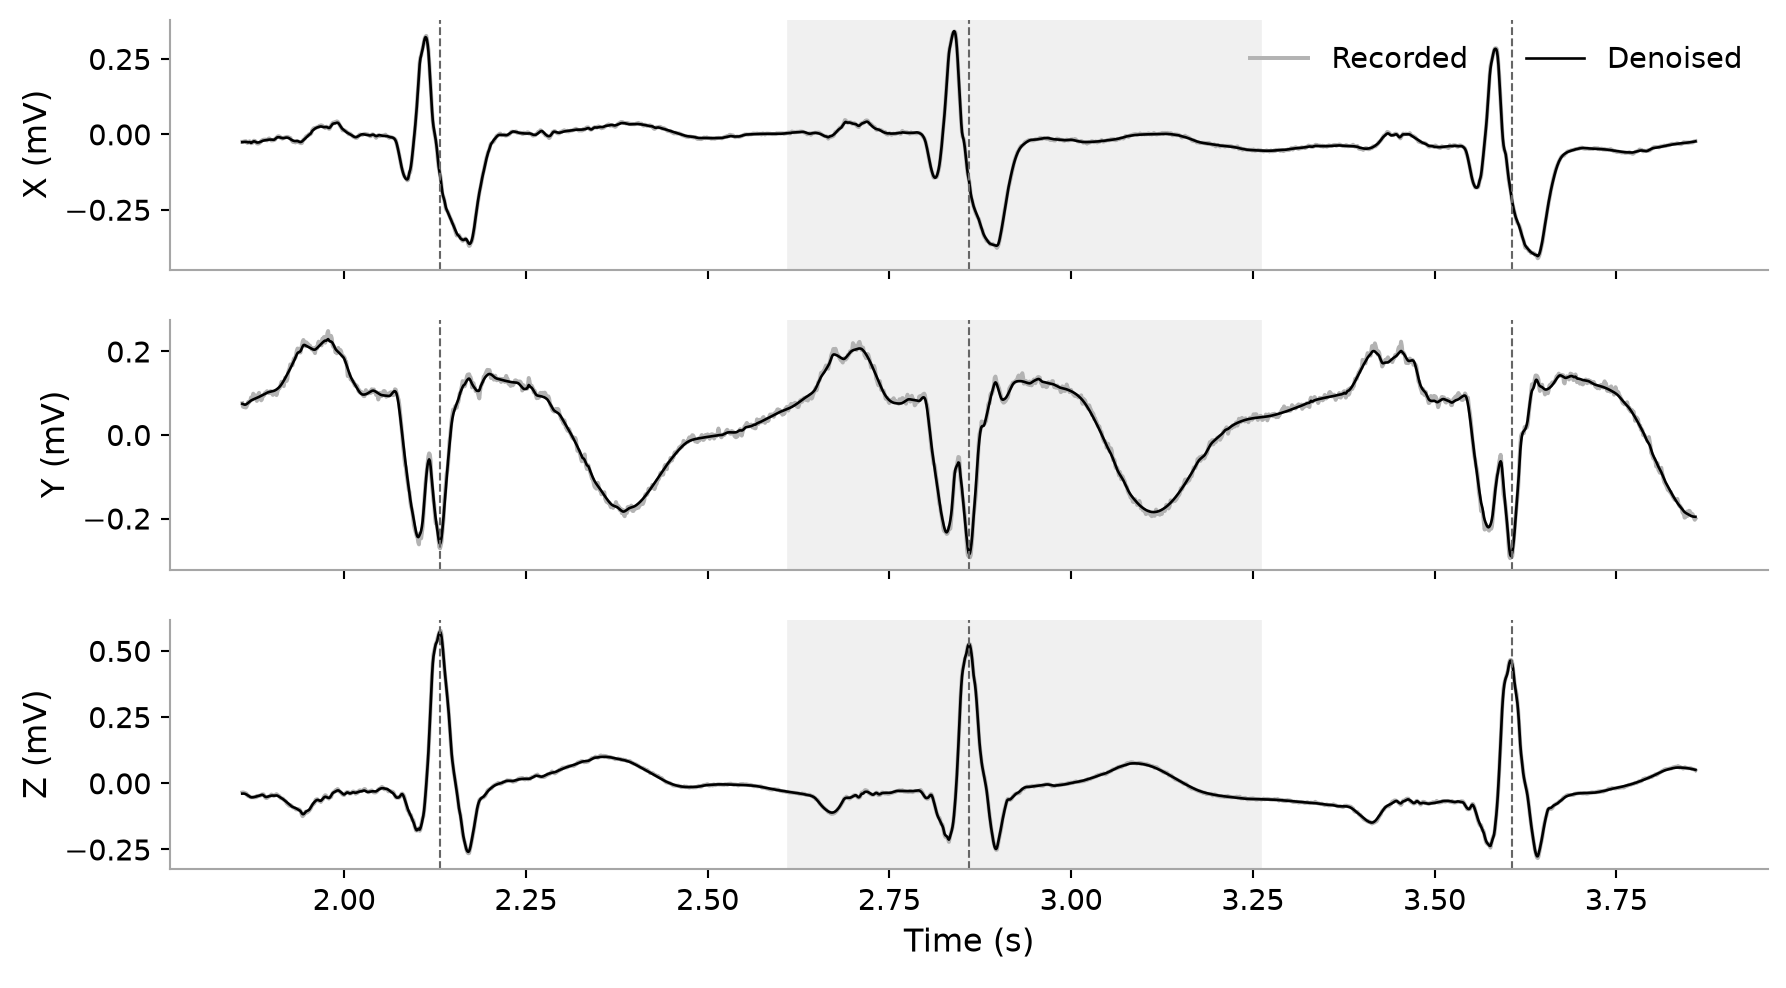
\includegraphics[width=\linewidth,height=4.9cm,keepaspectratio]{assets/vcg_processing_grayscale.png}
    \end{column}
    \begin{column}{0.29\textwidth}
      \small
      \textbf{Wavelet denoising}\\
      bior6.8 wavelet.
      \medskip

      \textbf{R-peak detection}\\
      Pan--Tompkins-style detector on vector magnitude.
      \medskip

      \textbf{Beat window}\\
      250 samples before R and 400 after R, including R.
      \medskip

      \textbf{651 samples per lead}
    \end{column}
  \end{columns}
  \sources{Real PTB record patient001/s0010\_re. Dashed lines: detected peaks. Shading: one beat.}
  \note{The pale trace is recorded VCG and the black trace is denoised VCG.
  The three panels show X, Y and Z. The detector uses their vector magnitude.
  The shaded interval is one 651-sample beat. This figure illustrates our
  processing output; it is not independent beat-annotation validation.
  The detector threshold of 0.06 was calibrated to published beat counts.
  Evidence: signal.py and configs/paper.yaml.
  Suggested time: 55 seconds. Transition: tensor construction.}
\end{frame}

% 5 -------------------------------------------------------------------
\begin{frame}{Tensor construction and Tucker features}
  \begin{enumerate}
    \item Retain the original beat and reconstruct details D3--D9.
    \item Construct the lead $\times$ time $\times$ subband tensor:
      \[\mathcal{X}\in\mathbb{R}^{3\times651\times8}.\]
    \item Compress only time to rank 3 using truncated SVD:
      \[\mathcal{G}\in\mathbb{R}^{3\times3\times8},
        \qquad \mathbf{f}=\operatorname{vec}(\mathcal{G})\in\mathbb{R}^{72}.\]
    \item Classify with a 500-tree bootstrap random forest.
  \end{enumerate}
  \sources{Lead and subband modes remain intact. SVD sign handling and flattening are deterministic.}
  \note{There are eight slices: the original signal plus seven details.
  We compress the time mode and retain the lead and subband modes.
  The core therefore gives 72 features per beat. The scikit-learn forest is
  an analogue of MATLAB TreeBagger. We use column-major core flattening.
  Evidence: features.py, evaluation.py and configs/paper.yaml.
  Suggested time: 60 seconds. Transition: reproduction results.}
\end{frame}

% 6 -------------------------------------------------------------------
\begin{frame}{The evaluation split changes the result}
  \begin{center}
    \begin{tabular}{lr}
      \toprule
      \textbf{12-class evaluation} & \textbf{Beat accuracy}\\
      \midrule
      Published paper & 99.80\%\\
      Our random beat 10-fold CV & 99.136\%\\
      Our patient-grouped 10-fold CV & 41.385\%\\
      \bottomrule
    \end{tabular}
  \end{center}
  \medskip
  \begin{itemize}
    \item Random beat folds put beats from the same patient on both sides.
    \item Patient grouping keeps every patient's beats and recordings together.
    \item The same baseline loses \textbf{57.75 percentage points} when test patients are unseen.
  \end{itemize}
  \sources{Both reproduced scores measure beat accuracy. Patient overlap is zero in grouped CV.}
  \note{Our random beat score is only 0.664 percentage points below the
  published accuracy. Almost every patient contributes to both training
  and testing in random beat folds. Patient grouping changes the
  generalization question. This is the main finding behind our project.
  We do not claim that this proves misconduct or invalidates every aspect
  of the paper. Evidence: RESULTS.md and the two saved metrics JSON files.
  Suggested time: 65 seconds. Transition: the six-class patient benchmark.}
\end{frame}

% 7 -------------------------------------------------------------------
\begin{frame}{Patient benchmark design}
  \begin{columns}[T,onlytextwidth]
    \begin{column}{0.30\textwidth}
      \centering
      \begin{tabular}{lr}
        \toprule
        \textbf{Class} & \textbf{Patients}\\
        \midrule
        AMI & 17\\ ALMI & 16\\ ASMI & 27\\
        IMI & 29\\ ILMI & 23\\ HC & 52\\
        \midrule
        Total & 164\\
        \bottomrule
      \end{tabular}
    \end{column}
    \begin{column}{0.65\textwidth}
      \begin{itemize}
        \item Six classes with at least 10 patients each.
        \item 164 patients and 55,863 beats.
        \item 10 outer patient folds and 3 inner folds for tuning.
        \item Equal class weights and equal patient weights within each class.
        \item Average beat probabilities to make one patient prediction.
      \end{itemize}
      \medskip
      \textbf{Primary endpoint: patient macro F1.}
    \end{column}
  \end{columns}
  \sources{Every outer fold contains all six classes. Inner tuning uses only training patients.}
  \note{Some original classes have one patient and cannot be learned when
  that patient is held out. The six-class endpoint addresses this issue.
  Macro F1 gives equal weight to the six class F1 scores. The folds are
  fixed in configs/patient\_folds.csv. Evidence: BENCHMARK\_RESULTS.md
  and benchmark.py. Suggested time: 60 seconds.
  Transition: comparison of classifiers on the same features.}
\end{frame}

% 8 -------------------------------------------------------------------
\begin{frame}{Classifier comparison on Tucker features}
  \begin{center}
    \begin{tabular}{lrr}
      \toprule
      \textbf{Model} & \textbf{Patient accuracy} & \textbf{Patient macro F1}\\
      \midrule
      Random forest & 47.56\% & 0.380\\
      Linear SVM & 43.90\% & 0.366\\
      XGBoost & 46.95\% & \textbf{0.403}\\
      \bottomrule
    \end{tabular}
  \end{center}
  \medskip
  \begin{itemize}
    \item Same 72 features, patient folds and nested selection protocol.
    \item XGBoost leads on the prespecified macro F1 endpoint.
    \item The bootstrap intervals overlap substantially.
  \end{itemize}
  \sources{Six-class PTB task. The current cohort does not establish a definitive classifier winner.}
  \note{Random forest has slightly higher accuracy, but the primary endpoint
  is macro F1. All three models remain limited on new patients.
  Evidence: BENCHMARK\_RESULTS.md and results/patient\_benchmark/.
  Suggested time: 45 seconds. Transition: changing the representation.}
\end{frame}

% 9 -------------------------------------------------------------------
\begin{frame}{Representation study with 12 ablations}
  \begin{center}
    \begin{tabular}{lrr}
      \toprule
      \textbf{Selected examples} & \textbf{Features} & \textbf{Patient macro F1}\\
      \midrule
      Wavelet statistics & 192 & \textbf{0.464}\\
      Tucker rank 5 & 120 & 0.423\\
      Tucker rank 3 & 72 & 0.416\\
      Amplitude-normalized Tucker & 72 & 0.369\\
      No wavelet subbands & 9 & 0.278\\
      \bottomrule
    \end{tabular}
  \end{center}
  \medskip
  \begin{itemize}
    \item Tested ranks, denoising, normalization, single leads and subbands.
    \item Wavelet statistics led the exploratory comparison.
    \item Same frozen folds and one fixed depth-6 XGBoost model.
  \end{itemize}
  \sources{Exploratory results differ from nested-selection estimates. All 12 results are in backup slide 16.}
  \note{An ablation changes the representation while holding evaluation
  fixed. Wavelet information and all three leads help in these comparisons.
  Additional Tucker rank yields modest gains. Evidence:
  ABLATION\_RESULTS.md and results/ablation/comparison.csv.
  Suggested time: 50 seconds. Transition: nested rerun of statistics.}
\end{frame}

% 10 ------------------------------------------------------------------
\begin{frame}{Wavelet statistics improved the PTB result}
  \[3\ \text{leads}\times8\ \text{slices}\times8\ \text{statistics}
    =192\ \text{features}.\]
  \small
  Mean, standard deviation, RMS, peak-to-peak amplitude, mean absolute value,
  log energy, skewness and kurtosis.
  \normalsize
  \medskip
  \begin{center}
    \begin{tabular}{lrr}
      \toprule
      \textbf{Nested PTB endpoint} & \textbf{Tucker + XGBoost} & \textbf{Statistics + XGBoost}\\
      \midrule
      Patient macro F1 & 0.403 & \textbf{0.487}\\
      Patient accuracy & 46.95\% & \textbf{54.88\%}\\
      \bottomrule
    \end{tabular}
  \end{center}
  \begin{itemize}
    \item Macro F1 gain: \textbf{+0.084}; paired 95\% interval: +0.003 to +0.165.
    \item Representation selection used these same PTB folds.
  \end{itemize}
  \sources{A nested rerun does not remove representation-selection bias. Fresh confirmation is required.}
  \note{The representation summarizes each lead and wavelet slice instead
  of compressing time into a Tucker core. The gain is encouraging within
  PTB, but selection happened after inspecting the ablations. Bootstrap
  uncertainty does not remove that selection effect. Evidence:
  ABLATION\_RESULTS.md and results/wavelet\_statistics\_confirm/.
  Suggested time: 65 seconds. Transition: external validation.}
\end{frame}

% 11 ------------------------------------------------------------------
\begin{frame}{Locked external validation on PTB-XL}
  \begin{itemize}
    \item Train on 164 eligible PTB patients and test once on PTB-XL fold 10.
    \item Strict test cohort: \textbf{1,185 records from 1,092 patients}.
    \item Convert 12-lead ECG to Kors-derived XYZ and resample 500 to 1,000 Hz.
    \item No PTB-XL model, threshold or representation tuning.
  \end{itemize}
  \medskip
  \begin{center}
    \begin{tabular}{lr}
      \toprule
      \textbf{External patient endpoint} & \textbf{Result}\\
      \midrule
      Model macro F1 & \textbf{0.242}\\
      Model accuracy & 56.23\%\\
      Always-healthy accuracy & 71.98\%\\
      \bottomrule
    \end{tabular}
  \end{center}
  \sources{Healthy controls are 72.0\% of this cohort. Localization does not transfer reliably.}
  \note{The strict label audit accepts one target MI location or isolated
  NORM and excludes ambiguous or conflicting patient status. The external
  cohort is imbalanced. Accuracy alone conceals weak localization, and
  ALMI has only five patients. Cross-database patient identity overlap is
  not independently verified. Evidence: EXTERNAL\_RESULTS.md and
  results/ptbxl\_external/metrics.json. Suggested time: 65 seconds.
  Transition: investigation of measured versus derived signals.}
\end{frame}

% 12 ------------------------------------------------------------------
\begin{frame}{Paired measured and derived VCG study}
  Same 164 PTB patients, 391 records and 55,863 original beat positions.
  \medskip
  \begin{center}
    \begin{tabular}{llr}
      \toprule
      \textbf{Training VCG} & \textbf{Test VCG} & \textbf{Patient macro F1}\\
      \midrule
      Measured Frank & Measured Frank & 0.469\\
      Measured Frank & Kors-derived & 0.422\\
      Kors-derived & Kors-derived & 0.467\\
      \bottomrule
    \end{tabular}
  \end{center}
  \begin{itemize}
    \item Estimated measured-to-derived change: \textbf{$-0.046$ macro F1}.
    \item Paired 95\% interval: $-0.108$ to $+0.017$, including zero.
    \item Conversion alone does not explain the external performance gap.
  \end{itemize}
  \sources{Fixed depth-3 XGBoost. Use the internal 0.469 control, not the earlier nested 0.487 estimate.}
  \note{Simultaneous ECG and measured Frank recordings allow a paired
  comparison that holds labels, patients and beat timing fixed. The
  directional pattern suggests a domain mismatch, but the effect size is
  uncertain. PTB-XL also changes device, recording length, labels and
  prevalence. Evidence: DOMAIN\_SHIFT\_RESULTS.md and paired metrics.
  Suggested time: 60 seconds. Transition: the reproducible codebase.}
\end{frame}

% 13 ------------------------------------------------------------------
\begin{frame}[fragile]{Codebase and reproducible experiments}
  \begin{columns}[T,onlytextwidth]
    \begin{column}{0.48\textwidth}
      \textbf{Python package}
      \begin{itemize}
        \item Data preparation and signal processing.
        \item Feature extraction and evaluation.
        \item Benchmarks and ablations.
        \item External and paired domain studies.
      \end{itemize}
    \end{column}
    \begin{column}{0.48\textwidth}
      \textbf{Repeatable experiments}
      \begin{itemize}
        \item Saved YAML settings and patient folds.
        \item Cached feature banks.
        \item Predictions, metrics and confusion matrices.
        \item \textbf{15 automated tests passing}.
      \end{itemize}
    \end{column}
  \end{columns}
  \medskip
  {\small
\begin{verbatim}
mi-localization run --mode both
mi-localization benchmark --models rf svm xgboost
\end{verbatim}
  }
  \sources{Repository: \url{https://github.com/Kumaryan12/major_project}. Large signals and model caches stay local.}
  \note{All experiments have fixed configurations and saved outputs.
  Feature caching avoids repeating preprocessing. The test suite covers
  signal/feature logic, benchmark behavior, label handling and external
  and domain workflows. The last verification gave 15 passing tests.
  Evidence: README.md, pyproject.toml, package sources and tests.
  Suggested time: 40 seconds. Transition: completed work and next steps.}
\end{frame}

% 14 ------------------------------------------------------------------
\begin{frame}{Completed work and next milestone}
  \begin{columns}[T,onlytextwidth]
    \begin{column}{0.48\textwidth}
      \textbf{Completed}
      \begin{itemize}
        \item Paper pipeline and close reproduction.
        \item Evaluation on unseen patients.
        \item Classifier and representation studies.
        \item External and paired domain experiments.
      \end{itemize}
    \end{column}
    \begin{column}{0.48\textwidth}
      \textbf{Proposed next milestone}
      \begin{itemize}
        \item Compact 1D CNN or ResNet.
        \item Tensor or wavelet features combined with learned features.
        \item Same patient endpoint and evaluation folds.
        \item Fresh independent confirmation.
      \end{itemize}
    \end{column}
  \end{columns}
  \medskip
  \textbf{The main contribution so far is a tested research baseline.}
  \sources{Current evidence does not establish state-of-the-art performance or clinical suitability.}
  \note{We have finished the reproduction and the additional studies.
  The proposed deep models and hybrid remain future work. Nearly matching
  high beat accuracy does not establish reliability on new patients.
  We should retain the patient endpoint and seek fresh validation for an
  improvement claim. Suggested time: 50 seconds. End the main talk here
  and invite questions. Slides 15--17 are backup material.}
\end{frame}

% Technical backup ----------------------------------------------------
\appendix

% 15 ------------------------------------------------------------------
\begin{frame}{Backup: class-level results}
  \begin{center}
    \begin{tabular}{lrrrr}
      \toprule
      \textbf{Class} & \textbf{PTB patients} & \textbf{Tucker F1} & \textbf{Statistics F1} & \textbf{External F1}\\
      \midrule
      AMI  & 17 & 0.188 & 0.357 & 0.049\\
      ALMI & 16 & 0.400 & 0.471 & 0.000\\
      ASMI & 27 & 0.412 & 0.373 & 0.380\\
      IMI  & 29 & 0.412 & 0.438 & 0.241\\
      ILMI & 23 & 0.263 & 0.450 & 0.035\\
      HC   & 52 & 0.742 & 0.835 & 0.747\\
      \bottomrule
    \end{tabular}
  \end{center}
  \begin{itemize}
    \item AMI and ILMI improve on PTB; ASMI declines.
    \item PTB and PTB-XL use different cohorts and label mappings.
    \item External ALMI has only five patients and zero correct classifications.
  \end{itemize}
  \sources{Patient-level class F1 from the nested PTB comparisons and fixed external test.}
  \note{Use this slide for class-specific questions. Improvement is not
  uniform. The external column is descriptive, not a controlled estimate
  of a single domain factor. Evidence: ABLATION\_RESULTS.md and
  EXTERNAL\_RESULTS.md.}
\end{frame}

% 16 ------------------------------------------------------------------
\begin{frame}{Backup: full exploratory ablation results}
  \small
  \renewcommand{\arraystretch}{1.04}
  \begin{center}
    \begin{tabular}{lrrr}
      \toprule
      \textbf{Representation} & \textbf{Features} & \textbf{Patient accuracy} & \textbf{Patient macro F1}\\
      \midrule
      Wavelet statistics & 192 & 53.66\% & 0.464\\
      Tucker rank 5 & 120 & 48.17\% & 0.423\\
      Tucker rank 8 & 192 & 49.39\% & 0.416\\
      Tucker rank 3 & 72 & 48.17\% & 0.416\\
      Raw signal, rank 3 & 72 & 47.56\% & 0.411\\
      Tucker rank 2 & 48 & 45.12\% & 0.377\\
      Amplitude normalized & 72 & 43.29\% & 0.369\\
      Z lead only & 24 & 42.68\% & 0.363\\
      Tucker rank 1 & 24 & 44.51\% & 0.353\\
      X lead only & 24 & 37.80\% & 0.320\\
      Y lead only & 24 & 35.37\% & 0.301\\
      No wavelet subbands & 9 & 35.37\% & 0.278\\
      \bottomrule
    \end{tabular}
  \end{center}
  \sources{Same frozen PTB folds and fixed depth-6 XGBoost. These are exploratory scores.}
  \note{This table records all twelve representations. Do not mix its
  scores with the nested selection scores. Evidence:
  results/ablation/comparison.csv and ABLATION\_RESULTS.md.}
\end{frame}

% 17 ------------------------------------------------------------------
\begin{frame}{Backup: technical choices and reproduction limits}
  \small
  \begin{tabularx}{\textwidth}{@{}p{0.25\textwidth}L@{}}
    \toprule
    \textbf{Choice} & \textbf{Implementation and limit}\\
    \midrule
    Wavelet boundaries & Symmetric extension and soft thresholding.\\
    R-peak detection & Vector magnitude; threshold 0.06 calibrated to beat counts.\\
    Feature determinism & SVD sign fixing and column-major core flattening.\\
    Classifier analogue & scikit-learn bootstrap forest instead of MATLAB TreeBagger.\\
    Exact replication & Unpublished annotations, folds and options limit exact matching.\\
    \bottomrule
  \end{tabularx}
  \par\medskip
  \textbf{Reference}\\
  Zhang et al., \textit{Automated Localization of Myocardial Infarction
  From Vectorcardiographic via Tensor Decomposition}, IEEE TBME,
  70(3), 812--823, 2023. DOI: 10.1109/TBME.2022.3202962.
  \sources{The code documents every implementation choice. Matching total beats does not match every annotation.}
  \note{These choices fill gaps in the publication. Nine wavelet levels
  on a 651-sample beat also make boundary handling consequential.
  Evidence: README.md reproduction boundaries, configs/paper.yaml and
  features.py. Use this slide for questions about exact replication.}
\end{frame}

\end{document}
